\chapter{LIS - Longest Increasing Subsequence}
Una Increasing Sequence (IS) è definita nel seguente modo:
\[ Z = <z_1, z_2, \dots, z_k> \]
Tale che $z_i < z_{i+1}$ per ogni indice i da 1 a k-1.
\paragraph*{Esempi}
\begin{align*}
    &<2,4,7,13,21> \rightarrow \text{ è una sequenza crescente}\\
    &<2> \rightarrow \text{ sequenza crescente}\\
    &<2,4,13,13,21> \rightarrow \text{ NON è una sequenza crescente}\\
    &<10,10,10> \rightarrow \text{ NON è una sequenza crescente}
\end{align*}
LIS di $X = <x_1, x_2, \dots, x_m>$ più lunga sottosequenza di X che sia
crescente. $Z = LIS(X)$.
\section{Esempio di LIS di X}  
    \[X= <14, 2, 4, 2, 7, 0, 13, 21, 11>\]
    \[LIS(X) = <2,4,7,13,21>\]
LIS è la più  lunga sottosequenza di X che sia crescente.
\subsection{Altro esempio}
\[X = <5, 4, 3, 2, 1>\]
\[LIS(X)=<5> \text{ or } <4> \text{ or } <3> \text{ or } <2> \text{ or } <1>\] 
\[X=<10, 10, 10, 10>\]
\[LIS(X) = 10 \]
\section{Definizione formale e identificazione tipologia problema}
\paragraph*{P:} Data una sequenza $X = <x_1, x_2, \dots, x_m>$ trovare la più lunga
sottosequenza crescente $Z=LIS(X)$.\\
\textbf{P è un problema di ottimizzazone di massimo, dove}:
\begin{itemize}
    \item (m) \ra dimensione del problema
    \item Soluzioni possibilie $\rightarrow$ tutte le sottosequenze crescenti di X
    \item Funzione obiettivo \ra lunghezza
    \item $|Z|$ è il valore ottimo del problema
    \item Z è una soluzione ottimale
\end{itemize}
\section{Soluzione}
\begin{enumerate}
    \item Calcolo dell'ottimo (lunghezza di Z)
    \item Ricostruzione di una soluzione ottimale
\end{enumerate}
\subsection{Definizione dei sottoproblemi - Primo tentativo}
\textbf{Sottoproblema di dimensione (i)}\\
Trovare la LIS del prefisso $X_i \rt LIS(X_i)$.\\
\textbf{Numero di sottoproblemi}: m+1.
Mentre per $i=m$ abbiamo il problema principale.
\subsection{Casi Base}
Sottoproblema di dimensione 0.\\
\[ i=0 \implies LIS(X_0) = <> \]
\subsection{Passo ricorsivo?}
\ra Tutti i sottoproblemi di dimensione (i) tale per cui $i > 0$.\\
\textbf{Qual è la sottostruttura ottima del problema?}\\
Proviamo la seguente sottostruttura:
\[LIS(X_m) = max\{LIS(X_{m-1}), LIS(X_{m-1})+<x_m>\}\]
\[X = <x_1, x_2, \dots, x_{m-1},x_m>\]
$LIS(X_m) = LIS(X_{m-1})+<x_m>$?
\begin{itemize}
    \item \textcolor{green}{Sì}, se $LIS(X_{m-1})$ finisce con un elmento $< x_m>$
    \item \textcolor{red}{No}, se $LIS(X_{m-1})$ finisce con un elemento $\geq x_m$
\end{itemize}
\subsection{Test sottostruttura - Primo tentativo}
Verifichiamo se la sottostruttura definita poco fa ci permette di trovare le LIS in
una stringa.
\paragraph*{Esempio} 
$ X = <14, 2, 4, 2, 7, 14, 15, 0, 13> \quad m=9$\\
$LIS(X_m) = LIS(X_{m-1})+<x_m>$? $x_m = 13$\\
$LIS(X_9) = LIS(X_8) + <13>$? $X=<14, 2, 4, 2, 7, 14, 15, 0, 13>$ \\
$LIS(X_9) = LIS(X_8) + <13> ?$\\
\textbf{NO!} Perchè risulta uguale a $<2, 4, 7, 14, 15> + <13> = <2, 4, 7, 14, 15, 13>$ e $15>13$, questo
significa che la sottostruttura non mi permette di avere una LIS.\\
Questo significa indica che mi manca dell'informazione, è necessario definire un problema
ausiliario che ci permette di creare una sottostruttura che trovi una LIS valida.
\section{Problema Ausiliario}
Si tratta di un sottoproblema di dimensione (i) che ha lo scopo di trovare la $LIS_v$ del
prefisso $X_i \rt LIS_v(X_i)$, $i \in \{1,2,\dots,m\}$.\\
Numero di sottoproblemi: m.\\
$LIS_V(X_m)$ \ra è la soluzione ottimale del problema ausiliario.\\
$LIS(X) \rt max\{LIS_V{X_i} \text{ t.c. } 1 \leq i \leq m\}$\\
Sostanzialmente cerco la LIS partendo dalla stringa base di 1 carattere, mano a mano
incremento di 1 e ricalcolo la LIS, fino ad arrivare a calcolare la LIS di tutta la stringa.
\paragraph*{Esempio}
\begin{align*}
    &X = <14, 2, 4, 2, 7, 14, 15, 0, 13>\\
    &LISV(X1) = <14>\\
    &LISV(X3) = <2, 4>\\
    &LISV(X2) = <2>\\
    &LISV(X5) = <2, 4, 7>\\
    &LISV(X6) = <2, 4, 7, 14>\\
    &LISV(X7) = <2, 4, 7, 14, 15> \quad \text{LIS(X)}\\
    &LISV(X8) = <0>\\
    &LISV(X9) = <2, 4, 7, 13>\\
    &LISV(X4) = <2>
\end{align*}
\subsection{Casi Base}
\ra Sottoproblema di dimensione (1).
\[i = 1 \implies LIS_V(X_1) = <x_1>\]
\subsection{Passo Ricorsivo}
\ra Tutti i sottoproblemi di dimensione (i) tale per cui $i >1$.\\
Qual è la sottostruttura ottima del problema Ausiliario?\\
\paragraph*{Esempio sottostruttura ottima}
\[X = <14, 2, 4, 2, 7, 14, 15, 0, 13, 21, 8> m = 11\]
\begin{align*}
    &LIS_V(X_{11}) \rt Z=<z_1, z_2, \dots, z_{k-1}, z_k> = <2,4,7,8>\\
    &z_k = x_{11} = 8\\
    &<z_1,z_2,\dots, z_{k-1}> \rt \text{ sottosequenza di }X_{10} \text{ per cui } z_{k-1}=x_5 = 7, \quad z_{k-1}<z_k\\
\end{align*}
Ottengo quindi che $<z_1,z_2,\dots, z_{k-1}> = LIS_V(X_5) + z_k = <2,4,7,8>$\\
\[LIS_V(X_5) = max\{LIS_V(X_h) \text{ t.c } 1 \leq h \leq 11, x_h < x_11\}\]
\[LISV(X_11) = max\{LIS_V(X_h) \text{ t.c. } 1 \leq h < 11, x_h < x_11\} + <x_11>\]
\subsection{Definizione sottostruttura ottima}
Data la sequenza $X=<x_1, x_2, \dots, x_m>$ e $LIS_V(X_m) = <z_1, z_2,\dots, x_{k-1}, z_k> = Z_{k-1} + <z_k>$:
\begin{align*}
    &z_k = x_m\\
    &Z_{k-1}=max\{LIS_V(X_h) \text{ t.c. } 1 \leq m, x_h < x_m\}\\
    &\text{ con max}\{\emptyset \} = <>
\end{align*}
\subsection{Passo ricorsivo (Problema Ausiliario - PA)}
Data la sequenza $X = <x_1, x_2, \dots, x_m>$:
\begin{align*}
    &LIS_V(X_m) = max\{LIS_V(X_h) \text{ t.c } 1 \leq h < m, x_h < x_m\}+ <x_m>\\ 
    &\text{ con max}\{\emptyset\}=<> \text{ che implica } LIS_V(X_m) = <x_m>
\end{align*}
Dato il prefisso $X_i = <x_1, x_2, \dots, x_i>:$
\begin{align*}
    &LIS_V(X_i) = max\{LIS_V(X_h) \text{ t.c } 1 \leq h < i, x_h < x_i\}+ <x_i>\\ 
    &\text{ con max}\{\emptyset\}=<> \text{ che implica } LIS_V(X_i) = <x_i>
\end{align*}
\subsection{Equazioni di ricorrenza - PA}
\paragraph*{i=1 (Caso Base)}
$LIS_V(X_1) = <x_1>$
\paragraph*{$i>1$ (Passo Ricorsivo)}
\begin{align*}
    &LIS_V(X_i) = max\{LIS_V(X_h) \text{ t.c. } 1 \leq h < i, \, x_h < x_j\} + <x_i>\\
    &\text{ con max}\{\emptyset\} = <> \, \text{ che implica } LIS_V(X_i)=<x_i>
\end{align*}
\subsection*{Definizione dei coefficienti - PA}
Coefficiente $c_i$ del sottoproblema (i):
\begin{align*}
    &c_i = |LIS_V(X_i)|\\
    &i \in \{1,2,\dots,m\}
\end{align*}
Numero di coefficienti: m.\\
$c_m = |LIS_V(X_m)| \rt$ valore ottimo di PA.
\subsection{Sostituzione coefficienti nelle equazioni di ricorrenza}
\paragraph*{i=1 (Caso Base)} $c_i = 1$
\paragraph*{$i>1$ (Passo Ricorsivo)}
\begin{align*}
    &c_i = max\{c_h \text{ t.c. } 1 \leq h < i, \, x_h < x_i\} + 1\\
    &\text{ con max}\{\emptyset\}=0 \text{ che implica } c_i = 1
\end{align*}
\subsection{Calcolo dell'ottimo (PA)}
\begin{itemize}
    \item Si calcolano i coefficienti $c_i$ per dimensione (i) crescente a partire dal
    caso base per $i=1$
    \item Si memorizza $c_i$ ogni volta che si risolve il sottoproblema (i)
    \item Quando si arriva a calcolare $c_m$ si ha il valore ottimo del problema ausiliario \ra
     $|LIS_V(X)|$
    \item Il valore ottimo del problema principale è dato da $max\{c_i \text{ t.c. }
     1 \leq i \leq m\} \rt |LIS(X)$
\end{itemize}
\subsection{Algoritmo DP (Bottom-up)}
\begin{itemize}
    \item Costruzione del vettore $C[1\dots m]$
    \item Riempimento di C in modo tale che $C[i]=c_i$
    \item Valore ottimo \ra massimo in C
\end{itemize}
%Slide 133 - Non ho molto capito la matrice ausiiaria
\subsection{Algoritmo DP (bottom-up)}
\begin{lstlisting}[language=Java, escapeinside={*@}{@*}]
    int calcolo_ottimo_LIS(X)
        C[1] = 1
        H[1] = 0
        valore_ottimo = C[1]
        for i from 2 to m do
            max = 0
            H[i] = 0
            for h from 1 to i-1 d
                if *@$x_h < x_i$@* and C[h] > max then
                    max = C[h]
                    H[i] = h
            C[i] = 1 + max
            if C[i] > valore_ottimo then
                valore_ottimo = C[i]
        return valore_ottimo
\end{lstlisting}
\subsection{Ricostruzione soluzione ottimale}
Mi basta leggere la matrice ausiliaria a partire dal valore massimo e vedere quando non ho 0 scrivere quello che ho in
corrispondenza della matrice.
\begin{center}
    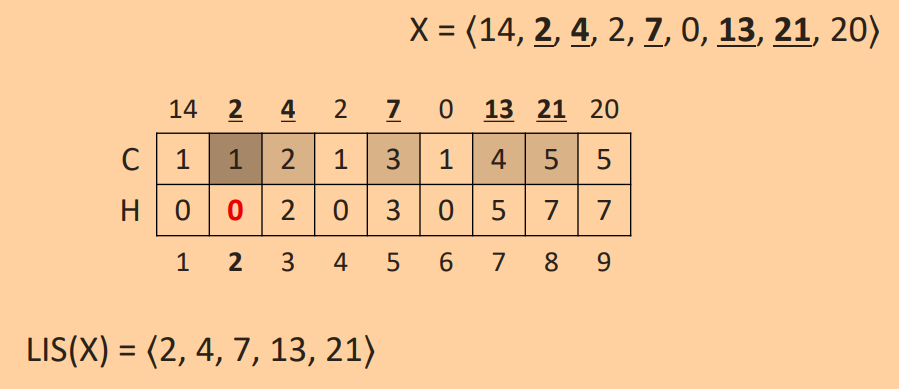
\includegraphics[width=70mm,scale=0.5]{chapters_ulerich/img/LIS_ricostruzione_sol_ott.png}
\end{center}
\subsection{Algoritmo di Ricostruzione - Ricorsivo}
\begin{lstlisting}[language=Java, escapeinside={*@}{@*}]
    Procedura ricostruisci_LIS_V(H, i)
        if H[i] != 0 then
            ricostruisci_LIS_V(H, H[i])
        print *@$x_i$@*
\end{lstlisting}
Chiamando la procedura per $i_{max}$ (posizione della cella
di C che contiene il valore massimo) si ottiene la
stampa di una soluzione ottimale di LIS(X).\\
Il caso peggiore sarà quando ho una stringa crescente, il tempo sarà di $O(m)$.\\
Il caso migliore invece è quando la stringa è decrescente, si ferma subito alla prima cella.
Avrò infatti $T$ costante.

        


